\subsubsubsubsection{Crossing}
\begin{figure}[h]
\centering
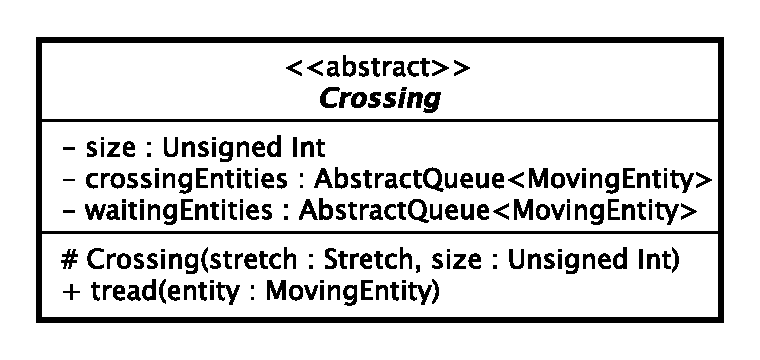
\includegraphics[scale=0.6,keepaspectratio]{images/solution/app/backend/crossing.eps}
\caption{\pReactiveComponentStretchDecoration::Crossing}
\label{fig:sd-app-crossing}
\end{figure}
\FloatBarrier
\begin{itemize}
  \item \textbf{\descr} \\
    It represents the zebra crossing entity. 
  \item \textbf{\attrs}
  \begin{itemize}
    \item \texttt{size: Unsigned Int} \\
The size of the stretch/\texttt{crossers} queue.
    \item \texttt{crossers: AbstractQueue<Traveller>} \\
The queue of travellers which are granted to cross the zebra crossing stretch.
  \item \texttt{incomers: AbstractQueue<Traveller>} \\
The queue of travellers which are currently waiting to cross the zebra crossing stretch.
  \end{itemize}
\item \textbf{\ops}
  \begin{itemize}
    \item[\#] \texttt{Crossing(stretch: Stretch, size: Unsigned Int)} \\
Creates a crossing with a specific component and two queues. The
\texttt{crossers} queue has a fixed size.
    \item[+] \texttt{tread(traveller: Traveller)} \\
Implements the treading of the stretch. This decoration allows all the
travellers in \texttt{crossers} to tread the crossing before any other traveller
which wants to tread the same stretches.
  \end{itemize}
\end{itemize}
